%!TEX root = ../dokumentation.tex

\chapter{Grundlagen}
\label{cha:Grundlagen}
In diesem Kapitel werden grundlegende Technologien und Systeme erklärt, welche im Rahmen dieser Arbeit Verwendung finden.


\section{DocBridge\textsuperscript{\textregistered} Mill Plus}{
\label{sec:MillPlus}
DocBridge\textsuperscript{\textregistered} Mill Plus ist eine plattformunabhängige, skalierbare Software für die Anzeige und Verarbeitung von Datenströmen. Sie ermöglicht die Analyse und Modifikation von Dokumenten in verschiedensten Formaten und die Konvertierung in unterschiedliche Ausgabeformate. Abbildung \ref{fig:compart_matrix} zeigt die unterstützten Formate. Die Dokumente lassen sich auf nahezu allen gängigen physikalischen und digitalen Kanälen darstellen. Mit DocBridge\textsuperscript{\textregistered} Mill Plus ist der Anwender auch dazu in der Lage, Prozesse die im Dokumentenmanagement üblich sind\footnote{Beispielsweise die Modifikation oder das Konvertieren von Dokumenten}, abzubilden. Der modulare Aufbau der Software lässt es zu, sie mit zusätzlichen Modulen um Ein- und Ausgabeformate sowie Workflows zu erweitern.

\begin{figure}[htbp] 
  \centering
     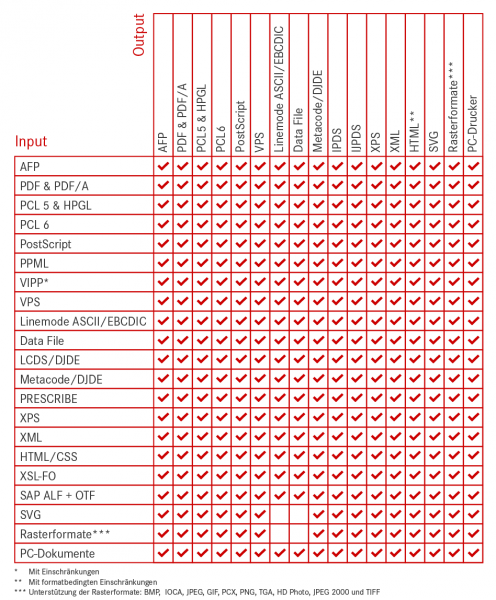
\includegraphics[height=.6\textwidth]{compart_matrix_de.png}
  \caption{Mögliche Verarbeitungsformate der DocBridge\textsuperscript{\textregistered} Mill Plus}
  \label{fig:compart_matrix}
\end{figure}

\newpage

}

\section{DocBridge\textsuperscript{\textregistered} Workbench for Mill Plus}{
\label{sec:DBWB}
DocBridge\textsuperscript{\textregistered} Workbench for Mill Plus bietet eine grafische Benutzeroberfläche für die Funktionalitäten der DocBridge\textsuperscript{\textregistered} Mill Plus wie Filterkonfigurationen und die Format-unabhängige Dokumentendarstellung. In der \ac{DBWB} können einzelne, mehrere oder in Stapeln zusammengefasste Dokumente angezeigt werden. Es werden alle in Abbildung \ref{fig:compart_matrix} aufgeführten Formate unterstützt. Geladene Dokumente können in der in Abbildung \ref{fig:dbwb_document} vorgestellten Dokumentenperspektive einheitlich dargestellt werden. Alle Dokumente, die in einem der unterstützten Formaten vorliegen, können im Anzeigebereich untersucht werden. So ist es dem Nutzer möglich, sich unabhängig vom Format des Dokuments, völlig auf dessen Inhalt zu konzentrieren. In der Prozessperspektive (Abbildung \ref{fig:dbwb_process}) können Verarbeitungsschritte konfiguriert, validiert und lokal ausgeführt werden. Die erstellte Prozesskonfiguration kann exportiert und in der DocBridge\textsuperscript{\textregistered} Mill Plus ausgeführt werden. Die Konfiguration der Prozesse erfolgt überwiegend über Drag \& Drop. Die Prozessperspektive ist die Standardperspektive der \ac{DBWB}.     

\newpage

\begin{figure}[htbp] 
\centering
     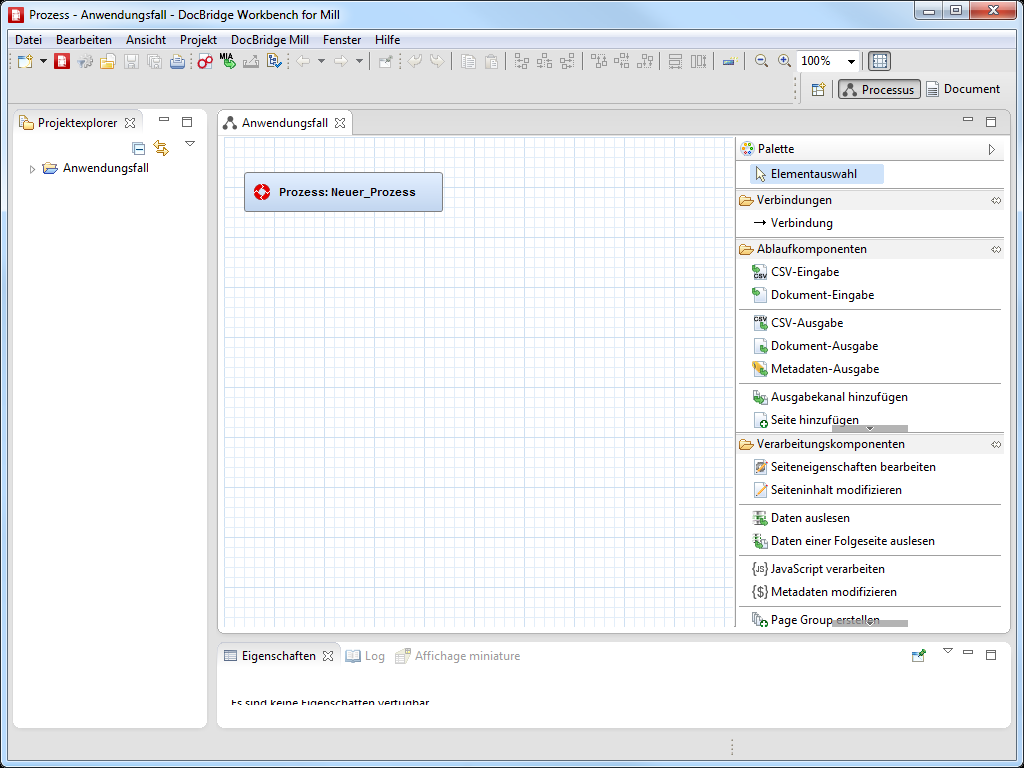
\includegraphics[height=.7\textwidth]{dbwb_process.png}
  \caption{Prozessperspektive}
  \label{fig:dbwb_process}
\end{figure}

\begin{figure}[htbp] 
\centering
     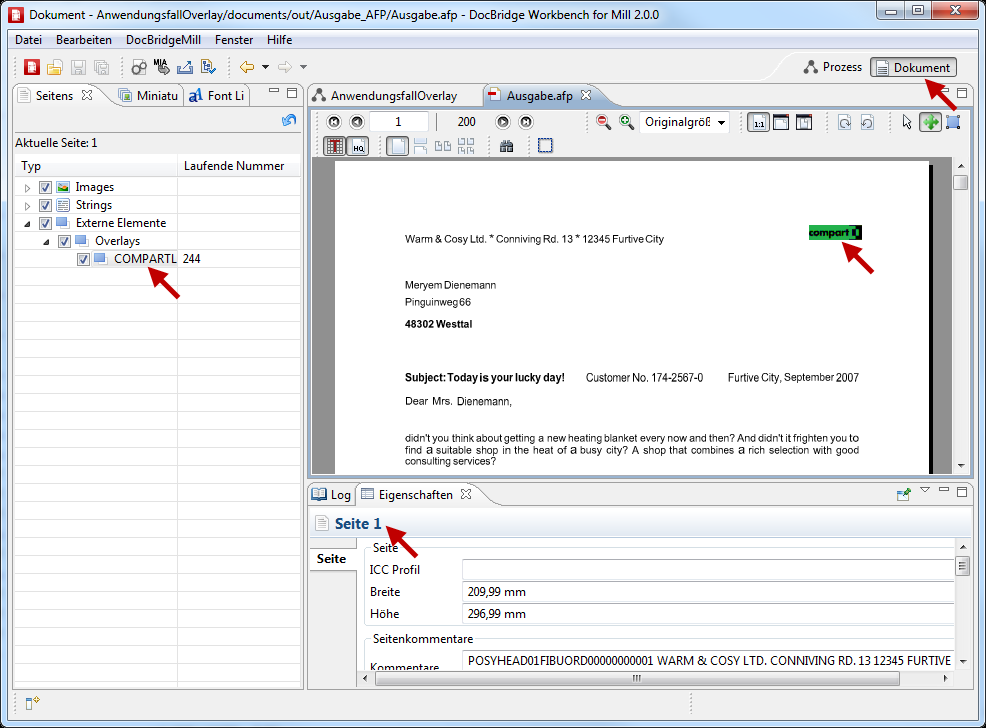
\includegraphics[height=.7\textwidth]{dbwb_document.png}
  \caption{Dokumentperspektive}
  \label{fig:dbwb_document}
\end{figure}


}
\newpage

\section{OSGi}{
\label{sec:OSGi}
Java stellt nur begrenzte Möglichkeiten zur Modularisierung bereit. "`Mit Modularisierung bezeichnet man die Aufteilung eines Softwaresystems in überschaubare Einzelteile, die jeweils einen abgeschlossenen Aufgabenbereich umfassen und untereinander mittels wohldefinierter Schnittstellen miteinander verbunden sind."' \cite[S.11]{rcp_unternehmenseinsatz} Java-Klassen lassen sich zwar unter der Verwendung von Packages gruppieren, jedoch ist es nicht möglich diese Gruppierungen und Restriktionen zur Laufzeit beizubehalten\cite[vgl. S.60]{RalfEbert}. Die Möglichkeit, einzelne Klassen als\\\texttt{package-protected} zu deklarieren ist "`für die
Strukturierung und Abgrenzung von Softwaremodulen meist unzureichend"'\cite[S.60]{RalfEbert}. \ac{OSGi} ermöglicht die Verwaltung der Sichtbarkeit von Packages zur Laufzeit. \ac{OSGi} ist ein Framework, welches sich auch dem Problem der Modularisierung annimmt und die Entwicklung von modularen Anwendungen auf der Java-Plattform ermöglicht. Abbildung \ref{fig:osgi_layer} zeigt das \ac{OSGi}-Schichtenmodell, das auf der \ac{JRE} aufsetzt. \ac{OSGi}-Anwendungen bestehen aus einzelnen Modulen, die auch Bundles genannt werden. Im Eclipse-Umfeld wird auch der Begriff "`Plug-in"' bedeutungsgleich für Bundles verwendet. Ein Bundle ist ein JAR-Archiv, das aus der Beschreibung des Bundles\footnote{Manifest.mf Datei}, Java-Klassen und Ressourcen besteht. Jedes Bundle hat einen eigenen Lebenszyklus. Dies bedeutet, dass zur Laufzeit einzelne Bundles dynamisch geladen und entfernt werden können. Die Spezifikation von \ac{OSGi} wird von der \ac{OSGi} Alliance erstellt. Die \ac{OSGi} Alliance wurde 1999 von rund 30 namhaften Firmen gegründet, um den Anforderungen im Bereich der eingebetteten Systeme gerecht zu werden \cite[vgl. S.3]{Queue}. Die Eclipse \ac{IDE} arbeitet seit Version 3.0 mit der \ac{OSGi} Implementierung Equinox.  Bei \ac{OSGi} Services handelt es sich um Java-Objekte, die unter einem Interface in der \ac{OSGi} Service-Registry angemeldet werden. In der Service-Registry angemeldete Services können von anderen Bundles verwendet werden. Services können genau wie OSGi-Bundles dynamisch geladen und entfernt werden. Wird ein Bundle, das einen Service bereitstellt gestoppt, so muss das verwendende Bundle auf das Wegfallen des Service entsprechend reagieren \cite[vgl. S.114]{OSGi}.
\begin{figure}[htbp] 
\centering
     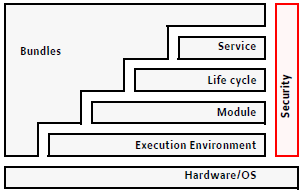
\includegraphics[height=.4\textwidth]{osgi_layer.png}
  \caption{OSGi Schichtenmodell \protect  \cite[aus S.2]{OSGi}}
  \label{fig:osgi_layer}
\end{figure}





}

\section{SWT}{
\label{sec:SWT}
Das Standard Widget Toolkit stellt das Framework für grafische Oberflächen auf der Eclipse-Plattform bereit. Diese grafischen Oberflächen sind aus Widgets aufgebaut. "`Traditionally, a widget is thought of as an abstract device that is useful for a particular purpose."'\cite[Kap.1]{SWT} \ac{SWT} stellt eine Java-Schnittstelle für die nativen GUI-Bibliotheken verschiedener Betriebssysteme zur Verfügung. Hierzu gehören Microsoft Windows, Linux\footnote{GIMP Toolkit} und Mac OS X\footnote{Cocoa}. Da auf die spezifischen Steuerelemente des jeweiligen Betriebssystems zugegriffen wird, kann mit \ac{SWT} auf den oben genannten Plattformen ein natives Aussehen und Verhalten erzielt werden, wie in Abbildung \ref{fig:swt_plattform} veranschaulicht wird.


\begin{figure}[htbp] 
  \centering
     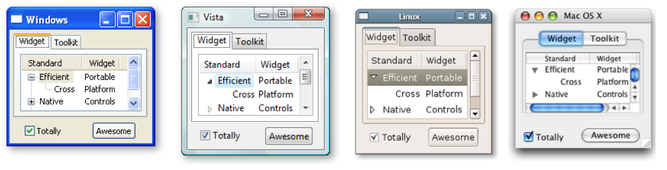
\includegraphics[height=.25\textwidth]{swt_plattform.png}
  \caption{Darstellung von SWT-Widgets auf verschiedenen Betriebssystemen \protect  \cite{RalfEbert}}
   \label{fig:swt_plattform}
\end{figure}




}

\section{Eclipse RCP}{
\label{sec:Eclipse_rcp}
Eclipse \ac{RCP} ist eine Plattform zur Entwicklung von Desktop-Anwendungen. Sie entstand aus der Eclipse \ac{IDE}, die sich aufgrund ihrer allgemeinen Natur anbot. Das Eclipse \ac{RCP}-Grundgerüst kann durch eigene Anwendungsfunktionalitäten erweitert werden. Viele der vorhandenen Komponenten können in eigenen Anwendungen genutzt werden. Als Beispiel wären hier Komponenten für eine Hilfe-Funktion oder das erweiterbare Plug-in-System zu nennen. Vorteile der Anwendungsentwicklung mit Eclipse \ac{RCP} sind die bereits vorhandenen Grundstrukturen für den Aufbau von GUI-Anwendungen und der modulare Aufbau. Dieser ermöglicht es, dass Erweiterungen auf Eclipse \ac{RCP}-Basis miteinander harmonieren. Die zur Implementierung benötigten Werkzeuge sind bereits in der Eclipse \ac{IDE}\footnote{Eclipse for RCP/Plug-in Developers} enthalten.
}

\section{Target Platform}{
\label{sec:target_plattform}
Eclipse \ac{RCP}-Applikationen werden für eine konfigurierbare Zielplattform\footnote{Target Platform} entwickelt. Alle externen Abhängigkeiten werden über die Target Platform geladen. Soll mit Plug-ins die Eclipse \ac{IDE} erweitert werden, verwendet man standardmäßig die Eclipse \ac{IDE} selbst als Target Platform \cite[vgl. S.14]{RalfEbert}. Bei der Entwicklung einer eigenen \ac{RCP}-Anwendung, oder Plug-ins für eine solche, ist das Verwenden der Eclipse \ac{IDE} "`unvorteilhaft, da die Eclipse-Installationen meist zu umfangreich sind und sich bei den einzelnen Entwicklern stark unterscheiden"'\cite[S.13]{eclipse_magazin}. In einem solchen Fall ist es günstiger, eine eigene Target Platform zu definieren. Durch die Definition der Target Platform kann festgelegt werden, in welcher Version der Applikation bestimmte Plug-ins eingebunden werden. Im Idealfall arbeiten alle Entwickler eines Projekts mit der selben Target Platform. So wird eine einheitliche Entwicklungsumgebung sichergestellt und Versionskonflikte vermieden.
}

\section{Apache Maven}{
\label{sec:apache_maven}
Das Tool Maven "`ist ein weiteres Top-Level-Projekt der \ac{ASE}. Sein Funktionsumfang ist etwas weiter gefasst als der von vergleichbaren Werkzeugen wie beispielsweise Ant, im Kern handelt es sich bei Maven aber um ein Werkzeug zur Durchführung eines Build-Prozesses"'\cite[S.75]{maven_popp}. Apache Maven basiert selbst auf Java und bietet die Möglichkeit, Java Programme standardisiert zu erstellen und zu verwalten. Mit Maven wird versucht, das Softwaredesign-Paradigma "Konvention vor Konfiguration"\footnote{Reduktion der Komplexität von Konfigurationen} für den gesamten Lebenszyklus der Softwareerstellung abzubilden. Dabei werden Schritte wie das Kompilieren und Testen so weit wie möglich automatisiert. Orientiert man sich bei der Entwicklung an den Maven Standards, ist es nur an wenigen Stellen nötig, Konfigurationen vorzunehmen.
}

\section{SonarQube\textsuperscript{\texttrademark}}{
\label{sec:soanr_qube}
Diese Plattform für statische Codeanalyse wird zur Sicherung der Codequalität eingesetzt. SonarQube\textsuperscript{\texttrademark}selbst ist wie Maven in Java implementiert, unterstützt jedoch eine Vielzahl von Programmiersprachen. Neben Java werden unter anderem die Sprachen C\#, C/C++, PL/SQL und Cobol unterstützt. SonarQube\textsuperscript{\texttrademark}analysiert Sourcecode auf Fehler oder unsaubere Programmierung und protokolliert die Ergebnisse in eine Datenbank. Auf einer Webseite werden die Ergebnisse der Analyse dargestellt. SonarQube\textsuperscript{\texttrademark}wird auch als Eclipse-Plug-in ausgeliefert. Dieses Plug-in kann Java Projekte mit Projekten aus der SonarQube\textsuperscript{\texttrademark}Datenbank assoziieren. Es ermöglicht eine lokale Nutzung und somit ein schnelleres Feedback für den Entwickler. Plattformen wie SonarQube\textsuperscript{\texttrademark}sind von großer Bedeutung, um die Codequalität in großen Softwareprojekten zu gewährleisten.  
}


\section{Plug-in zur Profilkonvertierung}{
Vom Studierenden wurde während der letzten Praxiseinheit ein \gls{Plug-in} im \ac{OSGi}-Umfeld entwickelt, welches dazu verwendet werden kann Filterprofile zu aktualisieren. Die Konfiguration von Konvertierungsabläufen wird in Filterprofilen festgehalten. Deren Aufbau ist in einem XML-Schema definiert. Kommen Funtionalitäten oder Komponenten bei der Filterkonfiguration hinzu, wird das Schema aktualisiert und somit abgeändert. Bestehende Filterprofile sind nun nicht mehr zum Schema valide. Das Plug-in zur Profilkonvertierung liest die Informationen aus dem alten Profil mit Hilfe von verschiedenen Java \ac{API}s aus und generiert anhand des Schemas ein neues Profil, das zum Schema valide ist. Sämtliche Inhalte werden dabei migriert. Es kommen vor allem die \ac{API}s  Jsoup\footnote{API zum Arbeiten mit degeneriertem HTML} und \ac{JaxB}\footnote{API für das Erstellen von Klassen aus einer XML-Schema-Instanz} zur Verwendung.
}

